
\begin{slide}{EXAFS: $\chi(k)$ and XAFS Fourier Transforms}

  \begin{cenpage}{140mm}

    EXAFS is an {\RedEmph{interference effect}}, using the wave-nature of
    the photo-electron.  We express the XAFS in terms of
    {\RedEmph{photo-electron wavenumber}}, ${k}$:

    \[  k= \sqrt{  \frac{2m(E-E_0)}{ {\hbar}^2} } \]

We'll also then use Fourier Transforms to convert from $k$ to  $R$.
\vmm



   \begin{columns}[T]
     \begin{column}{65mm}
       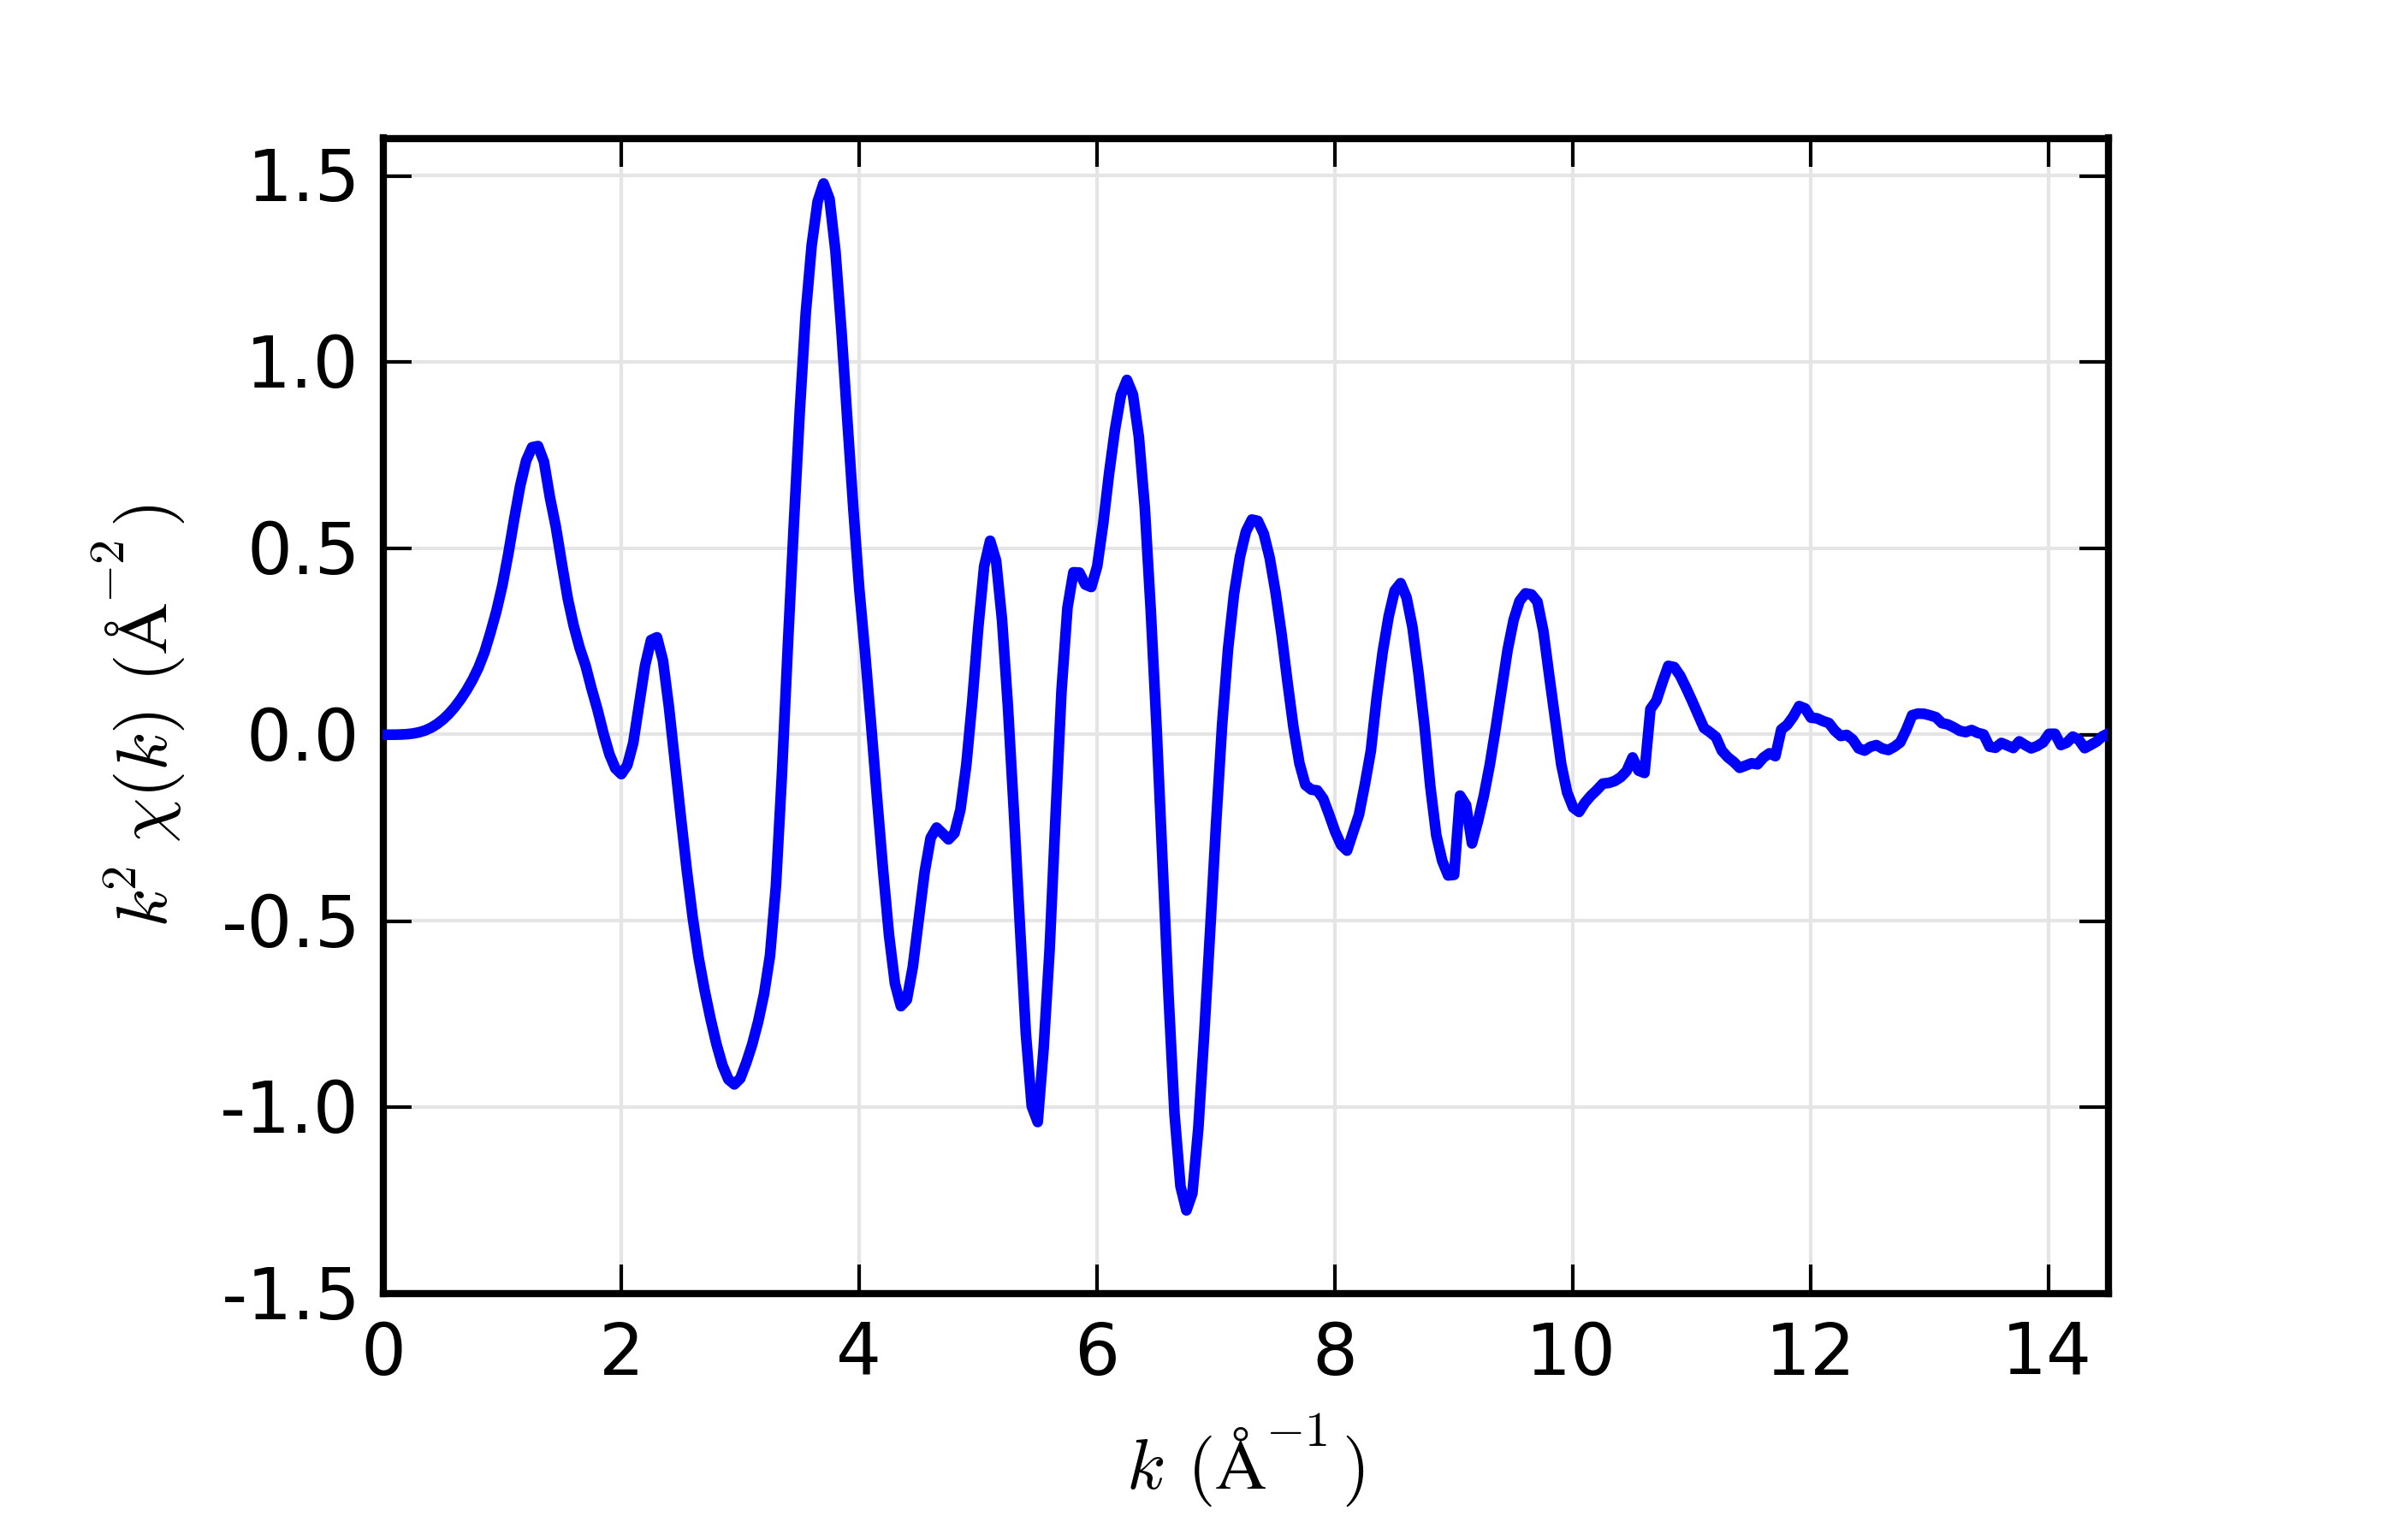
\includegraphics[width=58mm]{figs/rimg/feo_chik}
       \hspace{10mm} $k^2\chi(k)$ for FeO       
     \end{column}
     \begin{column}{65mm}
       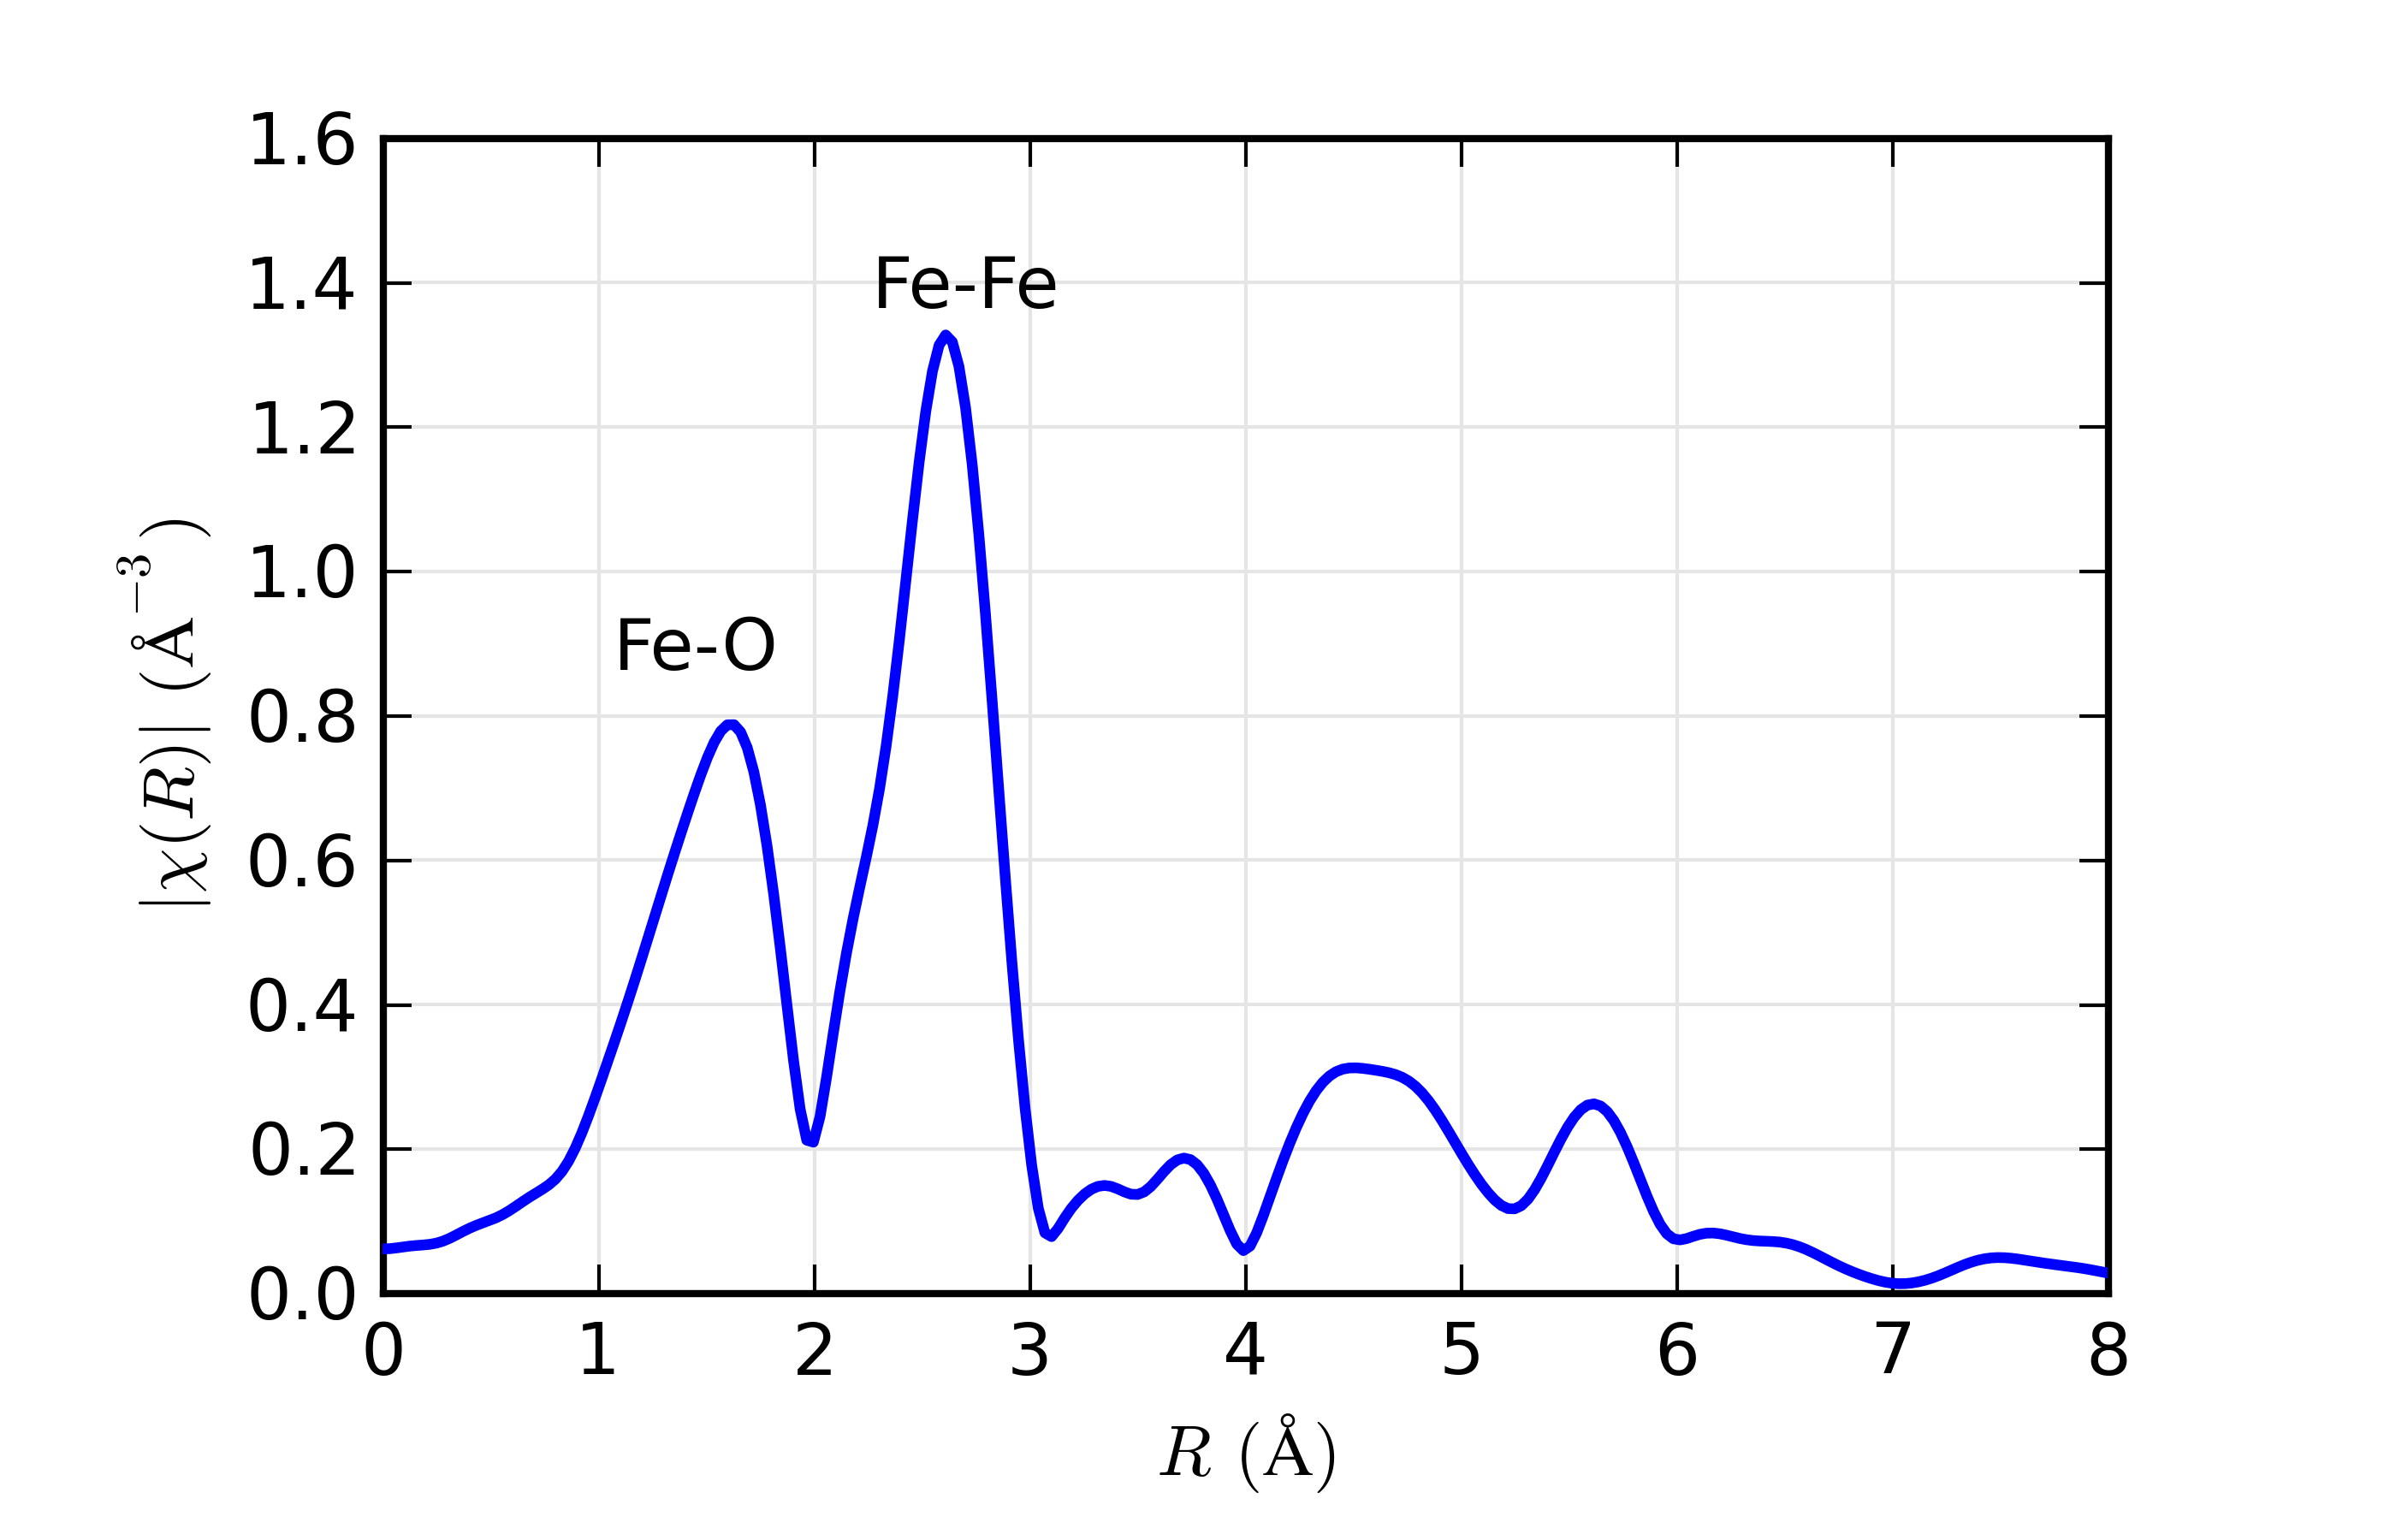
\includegraphics[width=58mm]{figs/rimg/feo_chir}
       \hspace{10mm}   Fourier Transform $|\chi(R)|$ for FeO. \par
       Similar to a Pair Distribution Function.
       
     \end{column}     
   \end{columns}


\end{cenpage}

\end{slide}
